\section{Test and evaluation of client-server communication}
To be certain that our client server communication works as it should, we will do both "real-life" practical tests and black-box testing, e.g. making sure the client and server behaves as it should on different occasions.

\subsection{Connection between client and server}
To make sure that the client(s) can connect to our server we have tested it in the following ways.
\begin{itemize}
	\item From local host, we started the server from the IntelliJ IDE and afterwards we started the client from Android Studio and connected to the server. In IntelliJ we could see that the server accepted the connection. Which is shown in \figref{fig:serverrunning}.
		\begin{figure}[h!]
  \centering
	    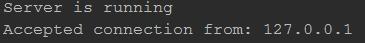
\includegraphics[width=0.6\textwidth]{figures/serverrunning.png}
    \caption{Server running and accepting connection}
    \label{fig:serverrunning}
\end{figure}
\end{itemize}
\begin{itemize}
	\item We downloaded the application to five smartphones and connected to the server, which the server handled correctly. We also requested a route on each smartphone and all of the smartphones received the same route. The time we had to wait for all of the smartphones to get the routes was between 19-24 minutes, which of course is not acceptable, but performance has not been a concern in this project.
\end{itemize}

\subsection{Message received matches the message sent}
To be certain the longitude, latitude and speed that is sent is received correctly on the server. We did the following test:
\begin{itemize}
	\item We gave the emulator in Android Studio a specific longitude and latitude and then used the application to send the data to the server. In IntelliJ's prompt window we got the following information displayed in \figref{fig:datasentfromclienttoserver}. Which confirms that the message sent from the client is received correctly on the server.
	\begin{figure}[h!]
  \centering
    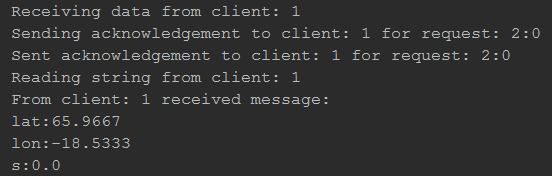
\includegraphics[width=0.8\textwidth]{figures/datasentfromclienttoserver.png}
    \caption{Data received on the server from the client}
    \label{fig:datasentfromclienttoserver}
\end{figure}
\end{itemize}

\subsection{If a message is lost}
To be sure that if some message is lost or connection between the client and server is not stable, which we also described in \autoref{chap:clientserver}, we are sending acknowledgements between client server. As  \figref{fig:datasentfromclienttoserver} illustrates when the server receives data from the client the server responds with an acknowledgement message to the client, that it has received the data.

\subsection{If server is down}
The user of the application has to be notified if they cant receive or send their data to the server. This is handled by giving a pop-up message to the user of the application that there is no connection to the server.

\subsection{GPS location and speed}
The location of the client and the speed it is moving at has been tested in a car with one person driving the car and another using a smartphone, where the smartphone displays the current speed and the location after a click on a button. The speed was compared to the car's speedometer which matched and the GPS location that was shown was later checked on a map, where the locations given by the smartphone also were correct.
\\
By doing these tests we have achieved the criteria listed in \autoref{chap:solutioncriteria}.